% Written by projects/think-time-rapid/paper/generate.mjs; do not edit by hand.

\newcommand{\AppCommit}{d8b771238c}
\newcommand{\Month}{2026-09}
\newcommand{\WindowLo}{1250}
\newcommand{\WindowHi}{1449}
\newcommand{\MinClock}{60}
\newcommand{\Strata}{five}
\newcommand{\Draws}{2,000}
\newcommand{\Seed}{20261014}
\newcommand{\Plateau}{60}
\newcommand{\BarShare}{80}
\newcommand{\DefendingPawns}{3}
\newcommand{\EarlyOwn}{four}
\newcommand{\WindowCentre}{1350}
\newcommand{\RatingLo}{900}
\newcommand{\RatingHi}{2099}
\newcommand{\Rushed}{10}
\newcommand{\Deep}{30}
\newcommand{\BookEnd}{45}
\newcommand{\Decided}{5}
\newcommand{\GamesRead}{6,185,560}
\newcommand{\GamesRapid}{1,019,414}
\newcommand{\GamesWithEvals}{195,409}
\newcommand{\GamesKept}{74,000}
\newcommand{\GamesBuilt}{74,000}
\newcommand{\BlackChecked}{800}
\newcommand{\MovesTimed}{4,721,351}
\newcommand{\MovesAnalysed}{3,738,138}
\newcommand{\MovesPrimary}{980,946}
\newcommand{\PlayerGames}{39,902}
\newcommand{\PrimaryQuick}{668,544}
\newcommand{\PrimaryLong}{54,331}
\newcommand{\LongShare}{6}
\newcommand{\QuickShare}{68}
\newcommand{\KeptTable}{%
\begin{tabular}{lrrrrrrr}
\toprule
mean rating & 800--999 & 1000--1199 & 1200--1399 & 1400--1599 & 1600--1799 & 1800--1999 & 2000--2199 \\
\midrule
games & 6,000 & 8,000 & 20,000 & 20,000 & 8,000 & 6,000 & 6,000 \\
\bottomrule
\end{tabular}
}
\newcommand{\AucQuick}{0.799}
\newcommand{\AucOther}{0.762}
\newcommand{\Trees}{400}
\newcommand{\SeriousQuick}{10.9}
\newcommand{\TriggerTable}{%
\begin{tabular}{lrrrrrllr}
\toprule
 & per & \multicolumn{2}{c}{moves} & \multicolumn{2}{c}{serious errors} & & & Holm \\
\cmidrule(lr){3-4}\cmidrule(lr){5-6}
moment & game & quick & long & quick & long & $\Delta$ & $\Delta - \Delta_{\text{none}}$ & $p$ \\
\midrule
Book end & 1.0 & 33,996 & 437 & 5.0 & 12.1 & $+$1.6 {\footnotesize ($-$0.1, $+$3.4)} & $-$3.1 {\footnotesize ($-$4.9, $-$1.2)} & 0.008 \\
Conversion & 5.3 & 134,722 & 13,192 & 11.9 & 23.4 & $+$8.8 {\footnotesize ($+$8.2, $+$9.5)} & $+$4.1 {\footnotesize ($+$3.3, $+$5.0)} & 0.004 \\
Forcing & 11.2 & 306,030 & 24,636 & 13.0 & 26.9 & $+$7.6 {\footnotesize ($+$7.1, $+$8.0)} & $+$2.9 {\footnotesize ($+$2.1, $+$3.6)} & 0.004 \\
Structure & 0.2 & 4,871 & 307 & 9.7 & 13.7 & $+$0.6 {\footnotesize ($-$2.3, $+$3.7)} & $-$4.1 {\footnotesize ($-$6.9, $-$1.0)} & 0.010 \\
\midrule
none & 7.0 & 188,925 & 15,759 & 11.0 & 23.1 & $+$4.7 {\footnotesize ($+$4.1, $+$5.3)} &  &  \\
\bottomrule
\end{tabular}
}
\newcommand{\BookEndDelta}{$+$1.6}
\newcommand{\BookEndLo}{$-$0.1}
\newcommand{\BookEndHi}{$+$3.4}
\newcommand{\BookEndVsNone}{$-$3.1}
\newcommand{\BookEndVsNoneLo}{$-$4.9}
\newcommand{\BookEndVsNoneHi}{$-$1.2}
\newcommand{\BookEndPHolm}{0.008}
\newcommand{\BookEndPerGame}{1.0}
\newcommand{\BookEndVerdict}{no sign it pays}
\newcommand{\BookEndThinkGap}{44}
\newcommand{\BookEndRateQuick}{5.0}
\newcommand{\BookEndRateLong}{12.1}
\newcommand{\BookEndDropped}{0.0}
\newcommand{\BookEndSaved}{$-$0.021}
\newcommand{\BookEndSavedLo}{$-$0.047}
\newcommand{\BookEndSavedHi}{0.002}
\newcommand{\ConversionDelta}{$+$8.8}
\newcommand{\ConversionLo}{$+$8.2}
\newcommand{\ConversionHi}{$+$9.5}
\newcommand{\ConversionVsNone}{$+$4.1}
\newcommand{\ConversionVsNoneLo}{$+$3.3}
\newcommand{\ConversionVsNoneHi}{$+$5.0}
\newcommand{\ConversionPHolm}{0.004}
\newcommand{\ConversionPerGame}{5.3}
\newcommand{\ConversionVerdict}{no sign it pays}
\newcommand{\ConversionThinkGap}{41}
\newcommand{\ConversionRateQuick}{11.9}
\newcommand{\ConversionRateLong}{23.4}
\newcommand{\ConversionDropped}{0.0}
\newcommand{\ConversionSaved}{$-$0.128}
\newcommand{\ConversionSavedLo}{$-$0.137}
\newcommand{\ConversionSavedHi}{$-$0.118}
\newcommand{\ForcingDelta}{$+$7.6}
\newcommand{\ForcingLo}{$+$7.1}
\newcommand{\ForcingHi}{$+$8.0}
\newcommand{\ForcingVsNone}{$+$2.9}
\newcommand{\ForcingVsNoneLo}{$+$2.1}
\newcommand{\ForcingVsNoneHi}{$+$3.6}
\newcommand{\ForcingPHolm}{0.004}
\newcommand{\ForcingPerGame}{11.2}
\newcommand{\ForcingVerdict}{no sign it pays}
\newcommand{\ForcingThinkGap}{43}
\newcommand{\ForcingRateQuick}{13.0}
\newcommand{\ForcingRateLong}{26.9}
\newcommand{\ForcingDropped}{0.0}
\newcommand{\ForcingSaved}{$-$0.106}
\newcommand{\ForcingSavedLo}{$-$0.113}
\newcommand{\ForcingSavedHi}{$-$0.100}
\newcommand{\StructureDelta}{$+$0.6}
\newcommand{\StructureLo}{$-$2.3}
\newcommand{\StructureHi}{$+$3.7}
\newcommand{\StructureVsNone}{$-$4.1}
\newcommand{\StructureVsNoneLo}{$-$6.9}
\newcommand{\StructureVsNoneHi}{$-$1.0}
\newcommand{\StructurePHolm}{0.010}
\newcommand{\StructurePerGame}{0.2}
\newcommand{\StructureVerdict}{no sign it pays}
\newcommand{\StructureThinkGap}{44}
\newcommand{\StructureRateQuick}{9.7}
\newcommand{\StructureRateLong}{13.7}
\newcommand{\StructureDropped}{0.0}
\newcommand{\StructureSaved}{$-$0.008}
\newcommand{\StructureSavedLo}{$-$0.051}
\newcommand{\StructureSavedHi}{0.031}
\newcommand{\NoneDelta}{$+$4.7}
\newcommand{\NoneLo}{$+$4.1}
\newcommand{\NoneHi}{$+$5.3}
\newcommand{\NonePerGame}{7.0}
\newcommand{\NoneRateQuick}{11.0}
\newcommand{\NoneRateLong}{23.1}
\newcommand{\NoneThinkGap}{41}
\newcommand{\Kept}{zero}
\newcommand{\NoSign}{four}
\newcommand{\CandidateTable}{%
\begin{tabular}{lrrrllrc}
\toprule
 & per & \multicolumn{2}{c}{moves} & & & Holm & \\
\cmidrule(lr){3-4}
before the move & game & quick & long & $\Delta$ & $\Delta - \Delta_{\text{none}}$ & $p$ & joins \\
\midrule
in check & 1.5 & 50,679 & 959 & $+$3.7 {\footnotesize ($+$1.7, $+$5.7)} & $-$1.0 {\footnotesize ($-$3.1, $+$1.0)} & 0.648 & no \\
after a capture & 6.3 & 194,911 & 9,034 & $+$8.2 {\footnotesize ($+$7.5, $+$8.9)} & $+$3.5 {\footnotesize ($+$2.6, $+$4.4)} & 0.008 & no \\
his piece hanging & 9.4 & 241,606 & 25,008 & $+$8.7 {\footnotesize ($+$8.2, $+$9.2)} & $+$4.0 {\footnotesize ($+$3.3, $+$4.7)} & 0.008 & no \\
opponent's piece hanging & 6.3 & 186,669 & 11,791 & $+$10.6 {\footnotesize ($+$9.9, $+$11.3)} & $+$5.9 {\footnotesize ($+$5.0, $+$6.8)} & 0.008 & no \\
after the opponent's error & 3.4 & 85,675 & 8,489 & $+$16.3 {\footnotesize ($+$15.1, $+$17.5)} & $+$11.6 {\footnotesize ($+$10.4, $+$12.8)} & 0.008 & no \\
defending, $-$3 or worse & 4.5 & 116,842 & 11,270 & $+$2.3 {\footnotesize ($+$1.9, $+$2.7)} & $-$2.4 {\footnotesize ($-$3.0, $-$1.8)} & 0.008 & no \\
book end and his next four & 4.8 & 159,050 & 4,040 & $+$4.6 {\footnotesize ($+$3.7, $+$5.5)} & $-$0.1 {\footnotesize ($-$1.0, $+$0.8)} & 0.901 & no \\
high danger, top fifth & 5.7 & 133,709 & 18,266 & $+$12.9 {\footnotesize ($+$12.2, $+$13.7)} & $+$8.2 {\footnotesize ($+$7.4, $+$9.1)} & 0.008 & no \\
\bottomrule
\end{tabular}
}
\newcommand{\CandidatesJoin}{zero}
\newcommand{\CandidatesPay}{zero}
\newcommand{\CandInCheckDelta}{$+$3.7}
\newcommand{\CandInCheckLo}{$+$1.7}
\newcommand{\CandInCheckHi}{$+$5.7}
\newcommand{\CandInCheckVsNone}{$-$1.0}
\newcommand{\CandInCheckPHolm}{0.648}
\newcommand{\CandAfterCaptureDelta}{$+$8.2}
\newcommand{\CandAfterCaptureLo}{$+$7.5}
\newcommand{\CandAfterCaptureHi}{$+$8.9}
\newcommand{\CandAfterCaptureVsNone}{$+$3.5}
\newcommand{\CandAfterCapturePHolm}{0.008}
\newcommand{\CandOwnHangingDelta}{$+$8.7}
\newcommand{\CandOwnHangingLo}{$+$8.2}
\newcommand{\CandOwnHangingHi}{$+$9.2}
\newcommand{\CandOwnHangingVsNone}{$+$4.0}
\newcommand{\CandOwnHangingPHolm}{0.008}
\newcommand{\CandOppHangingDelta}{$+$10.6}
\newcommand{\CandOppHangingLo}{$+$9.9}
\newcommand{\CandOppHangingHi}{$+$11.3}
\newcommand{\CandOppHangingVsNone}{$+$5.9}
\newcommand{\CandOppHangingPHolm}{0.008}
\newcommand{\CandAfterOppErrorDelta}{$+$16.3}
\newcommand{\CandAfterOppErrorLo}{$+$15.1}
\newcommand{\CandAfterOppErrorHi}{$+$17.5}
\newcommand{\CandAfterOppErrorVsNone}{$+$11.6}
\newcommand{\CandAfterOppErrorPHolm}{0.008}
\newcommand{\CandDefendingDelta}{$+$2.3}
\newcommand{\CandDefendingLo}{$+$1.9}
\newcommand{\CandDefendingHi}{$+$2.7}
\newcommand{\CandDefendingVsNone}{$-$2.4}
\newcommand{\CandDefendingPHolm}{0.008}
\newcommand{\CandEarlyDelta}{$+$4.6}
\newcommand{\CandEarlyLo}{$+$3.7}
\newcommand{\CandEarlyHi}{$+$5.5}
\newcommand{\CandEarlyVsNone}{$-$0.1}
\newcommand{\CandEarlyPHolm}{0.901}
\newcommand{\CandHighDangerDelta}{$+$12.9}
\newcommand{\CandHighDangerLo}{$+$12.2}
\newcommand{\CandHighDangerHi}{$+$13.7}
\newcommand{\CandHighDangerVsNone}{$+$8.2}
\newcommand{\CandHighDangerPHolm}{0.008}
\newcommand{\HighDangerCut}{20.2}
\newcommand{\BookEndBarPlot}{%
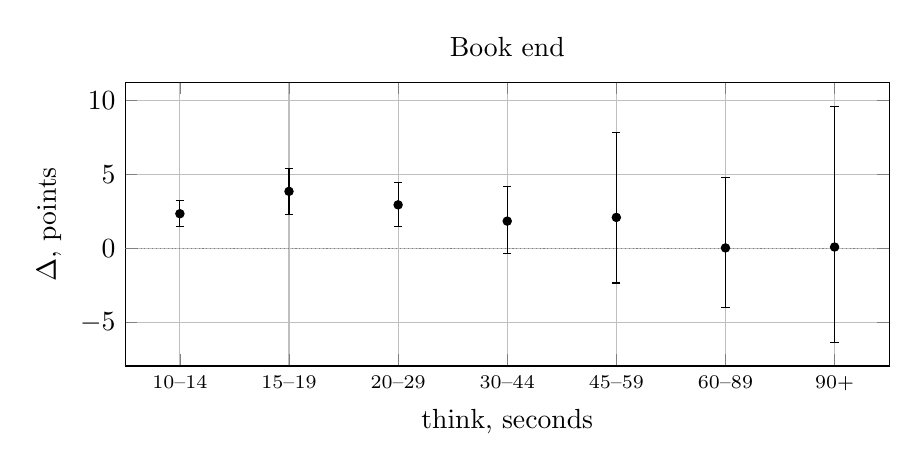
\begin{tikzpicture}
\begin{axis}[scale only axis, width=0.8\linewidth, height=3.6cm, title={Book end}, xtick={0,...,6}, xticklabels={10--14,15--19,20--29,30--44,45--59,60--89,90+},
  xmin=-0.5, xmax=6.5, x tick label style={font=\scriptsize}, ylabel={$\Delta$, points}, xlabel={think, seconds}, grid=major]
\addplot[only marks, mark=*, mark size=1.5pt, black, error bars/.cd, y dir=both, y explicit] coordinates {
(0, 2.34) += (0, 0.87) -= (0, 0.89)
(1, 3.85) += (0, 1.55) -= (0, 1.55)
(2, 2.94) += (0, 1.49) -= (0, 1.44)
(3, 1.84) += (0, 2.36) -= (0, 2.17)
(4, 2.09) += (0, 5.72) -= (0, 4.43)
(5, 0.03) += (0, 4.78) -= (0, 4.03)
(6, 0.09) += (0, 9.52) -= (0, 6.44)
};
\draw[gray, densely dotted] (axis cs:-1,0) -- (axis cs:7,0);
\end{axis}
\end{tikzpicture}
}
\newcommand{\ConversionBarPlot}{%
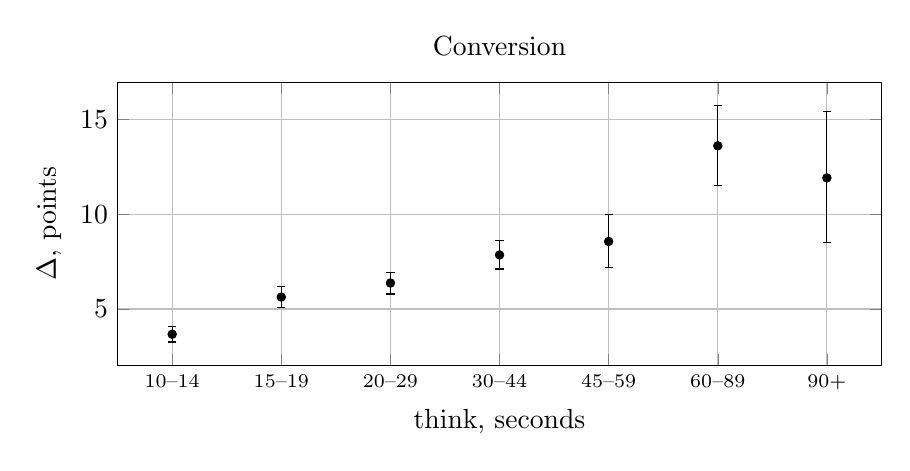
\begin{tikzpicture}
\begin{axis}[scale only axis, width=0.8\linewidth, height=3.6cm, title={Conversion}, xtick={0,...,6}, xticklabels={10--14,15--19,20--29,30--44,45--59,60--89,90+},
  xmin=-0.5, xmax=6.5, x tick label style={font=\scriptsize}, ylabel={$\Delta$, points}, xlabel={think, seconds}, grid=major]
\addplot[only marks, mark=*, mark size=1.5pt, black, error bars/.cd, y dir=both, y explicit] coordinates {
(0, 3.67) += (0, 0.40) -= (0, 0.41)
(1, 5.63) += (0, 0.56) -= (0, 0.54)
(2, 6.37) += (0, 0.56) -= (0, 0.58)
(3, 7.85) += (0, 0.77) -= (0, 0.74)
(4, 8.56) += (0, 1.40) -= (0, 1.35)
(5, 13.60) += (0, 2.11) -= (0, 2.09)
(6, 11.91) += (0, 3.51) -= (0, 3.41)
};
\draw[gray, densely dotted] (axis cs:-1,0) -- (axis cs:7,0);
\end{axis}
\end{tikzpicture}
}
\newcommand{\ForcingBarPlot}{%
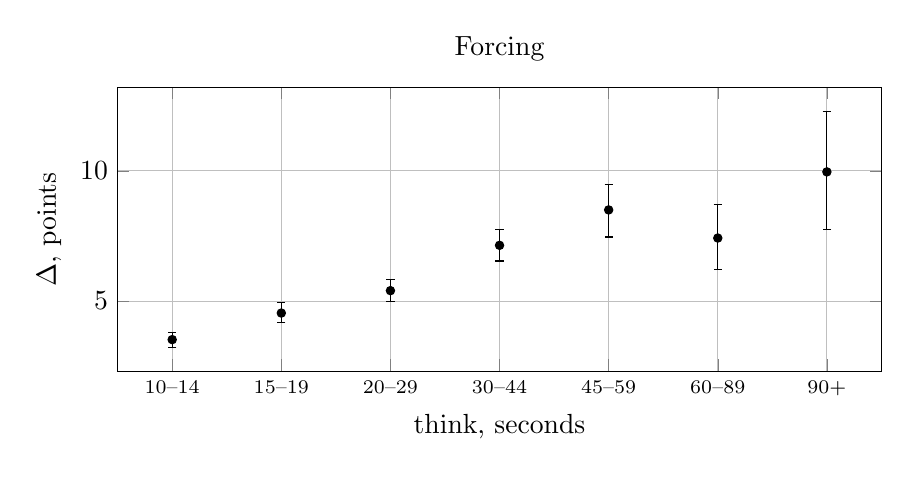
\begin{tikzpicture}
\begin{axis}[scale only axis, width=0.8\linewidth, height=3.6cm, title={Forcing}, xtick={0,...,6}, xticklabels={10--14,15--19,20--29,30--44,45--59,60--89,90+},
  xmin=-0.5, xmax=6.5, x tick label style={font=\scriptsize}, ylabel={$\Delta$, points}, xlabel={think, seconds}, grid=major]
\addplot[only marks, mark=*, mark size=1.5pt, black, error bars/.cd, y dir=both, y explicit] coordinates {
(0, 3.52) += (0, 0.29) -= (0, 0.30)
(1, 4.54) += (0, 0.40) -= (0, 0.37)
(2, 5.40) += (0, 0.42) -= (0, 0.43)
(3, 7.14) += (0, 0.60) -= (0, 0.60)
(4, 8.50) += (0, 0.98) -= (0, 1.04)
(5, 7.42) += (0, 1.28) -= (0, 1.22)
(6, 9.96) += (0, 2.33) -= (0, 2.20)
};
\draw[gray, densely dotted] (axis cs:-1,0) -- (axis cs:7,0);
\end{axis}
\end{tikzpicture}
}
\newcommand{\StructureBarPlot}{%
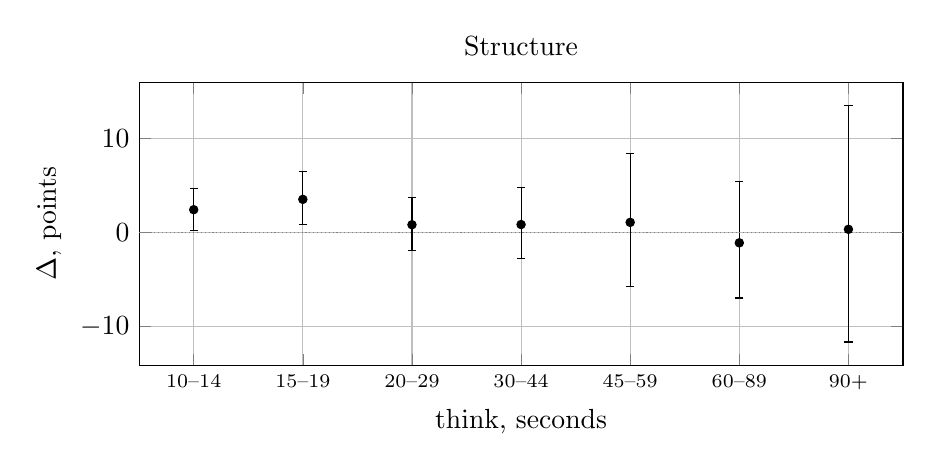
\begin{tikzpicture}
\begin{axis}[scale only axis, width=0.8\linewidth, height=3.6cm, title={Structure}, xtick={0,...,6}, xticklabels={10--14,15--19,20--29,30--44,45--59,60--89,90+},
  xmin=-0.5, xmax=6.5, x tick label style={font=\scriptsize}, ylabel={$\Delta$, points}, xlabel={think, seconds}, grid=major]
\addplot[only marks, mark=*, mark size=1.5pt, black, error bars/.cd, y dir=both, y explicit] coordinates {
(0, 2.41) += (0, 2.26) -= (0, 2.18)
(1, 3.51) += (0, 2.98) -= (0, 2.66)
(2, 0.81) += (0, 2.89) -= (0, 2.72)
(3, 0.83) += (0, 3.96) -= (0, 3.59)
(4, 1.06) += (0, 7.35) -= (0, 6.82)
(5, -1.12) += (0, 6.54) -= (0, 5.87)
(6, 0.32) += (0, 13.15) -= (0, 12.00)
};
\draw[gray, densely dotted] (axis cs:-1,0) -- (axis cs:7,0);
\end{axis}
\end{tikzpicture}
}
\newcommand{\BookEndPlateau}{$+$0.1}
\newcommand{\BookEndPlateauLo}{$-$3.4}
\newcommand{\BookEndPlateauHi}{$+$3.9}
\newcommand{\BookEndBar}{none}
\newcommand{\BookEndAppBar}{45}
\newcommand{\BookEndBarVerdict}{no bar}
\newcommand{\ConversionPlateau}{$+$13.3}
\newcommand{\ConversionPlateauLo}{$+$11.5}
\newcommand{\ConversionPlateauHi}{$+$15.1}
\newcommand{\ConversionBar}{none}
\newcommand{\ConversionAppBar}{30}
\newcommand{\ConversionBarVerdict}{no bar}
\newcommand{\ForcingPlateau}{$+$8.1}
\newcommand{\ForcingPlateauLo}{$+$7.0}
\newcommand{\ForcingPlateauHi}{$+$9.2}
\newcommand{\ForcingBar}{none}
\newcommand{\ForcingAppBar}{30}
\newcommand{\ForcingBarVerdict}{no bar}
\newcommand{\StructurePlateau}{$-$0.5}
\newcommand{\StructurePlateauLo}{$-$6.0}
\newcommand{\StructurePlateauHi}{$+$5.5}
\newcommand{\StructureBar}{none}
\newcommand{\StructureAppBar}{30}
\newcommand{\StructureBarVerdict}{no bar}
\newcommand{\Bars}{zero}
\newcommand{\TrendTable}{%
\begin{tabular}{llllll}
\toprule
mover's rating & none & book end & conversion & forcing & structure \\
\midrule
900--1099 & $+$5.3 {\footnotesize ($+$4.2, $+$6.4)} & $+$8.8 {\footnotesize ($+$4.3, $+$14.2)} & $+$10.0 {\footnotesize ($+$8.9, $+$11.1)} & $+$7.8 {\footnotesize ($+$6.9, $+$8.7)} & $+$1.1 {\footnotesize ($-$5.6, $+$7.6)} \\
1100--1299 & $+$4.9 {\footnotesize ($+$4.2, $+$5.6)} & $+$2.8 {\footnotesize ($+$0.7, $+$5.0)} & $+$8.7 {\footnotesize ($+$7.9, $+$9.4)} & $+$7.6 {\footnotesize ($+$7.0, $+$8.2)} & $+$3.9 {\footnotesize ($-$0.4, $+$8.3)} \\
1300--1499 & $+$4.6 {\footnotesize ($+$4.0, $+$5.1)} & $+$2.2 {\footnotesize ($+$0.3, $+$4.2)} & $+$8.9 {\footnotesize ($+$8.2, $+$9.6)} & $+$7.7 {\footnotesize ($+$7.2, $+$8.1)} & $-$0.1 {\footnotesize ($-$3.0, $+$3.1)} \\
1500--1699 & $+$4.5 {\footnotesize ($+$3.9, $+$5.1)} & $+$1.2 {\footnotesize ($-$0.7, $+$3.3)} & $+$8.8 {\footnotesize ($+$8.1, $+$9.6)} & $+$8.2 {\footnotesize ($+$7.6, $+$8.7)} & $+$3.8 {\footnotesize ($+$0.3, $+$7.5)} \\
1700--1899 & $+$5.0 {\footnotesize ($+$4.3, $+$5.7)} & $+$1.3 {\footnotesize ($-$0.8, $+$3.8)} & $+$8.9 {\footnotesize ($+$7.9, $+$10.0)} & $+$7.1 {\footnotesize ($+$6.4, $+$7.8)} & $-$3.0 {\footnotesize ($-$6.0, $+$0.5)} \\
1900--2099 & $+$4.0 {\footnotesize ($+$3.4, $+$4.6)} & $+$0.8 {\footnotesize ($-$1.0, $+$2.9)} & $+$8.8 {\footnotesize ($+$7.7, $+$9.9)} & $+$7.4 {\footnotesize ($+$6.8, $+$8.1)} & $+$5.8 {\footnotesize ($+$1.4, $+$10.7)} \\
\bottomrule
\end{tabular}
}
\newcommand{\SamePositions}{292}
\newcommand{\SameQuick}{9,974}
\newcommand{\SameLong}{386}
\newcommand{\SameDelta}{$+$1.9}
\newcommand{\SameLo}{$-$1.0}
\newcommand{\SameHi}{$+$5.0}
\newcommand{\SameCutBound}{1.0}
\newcommand{\SameBoards}{%
\begin{subfigure}[t]{0.32\textwidth}\centering
\chessboard[setfen={rnbqkbnr/ppp1pppp/8/3p4/3P1B2/8/PPP1PPPP/RN1QKBNR b KQkq - 0 1}, boardfontsize=11pt]
\caption*{Black to move: 655 quick moves, 0.0\% serious; 6 long, 0.0\%.\\[0.2em]\fen{rnbqkbnr/ppp1pppp/8/3p4/3P1B2/8/PPP1PPPP/RN1QKBNR b KQkq -}}
\end{subfigure}\hfill
\begin{subfigure}[t]{0.32\textwidth}\centering
\chessboard[setfen={r1bqkbnr/pppp1ppp/2n5/4p3/2B1P3/5N2/PPPP1PPP/RNBQK2R b KQkq - 0 1}, boardfontsize=11pt]
\caption*{Black to move: 477 quick moves, 6.9\% serious; 4 long, 0.0\%.\\[0.2em]\fen{r1bqkbnr/pppp1ppp/2n5/4p3/2B1P3/5N2/PPPP1PPP/RNBQK2R b KQkq -}}
\end{subfigure}\hfill
\begin{subfigure}[t]{0.32\textwidth}\centering
\chessboard[setfen={rnbqkbnr/pp1ppppp/8/2p5/4P3/8/PPPP1PPP/RNBQKBNR w KQkq - 0 1}, boardfontsize=11pt]
\caption*{White to move: 324 quick moves, 0.0\% serious; 1 long, 0.0\%.\\[0.2em]\fen{rnbqkbnr/pp1ppppp/8/2p5/4P3/8/PPPP1PPP/RNBQKBNR w KQkq -}}
\end{subfigure}
}
\newcommand{\SensitivityTable}{%
\begin{tabular}{lllll}
\toprule
 & \multicolumn{2}{c}{ten strata} & \multicolumn{2}{c}{quick from 6 seconds} \\
\cmidrule(lr){2-3}\cmidrule(lr){4-5}
moment & $\Delta$ & $\Delta - \Delta_{\text{none}}$ & $\Delta$ & $\Delta - \Delta_{\text{none}}$ \\
\midrule
Book end & $+$1.2 {\footnotesize ($-$0.4, $+$3.0)} & $-$3.6 {\footnotesize ($-$5.3, $-$1.8)} & $+$0.5 {\footnotesize ($-$1.7, $+$2.8)} & $-$3.5 {\footnotesize ($-$5.8, $-$1.2)} \\
Conversion & $+$8.8 {\footnotesize ($+$8.1, $+$9.4)} & $+$3.9 {\footnotesize ($+$3.1, $+$4.8)} & $+$7.2 {\footnotesize ($+$6.5, $+$8.0)} & $+$3.2 {\footnotesize ($+$2.3, $+$4.2)} \\
Forcing & $+$7.4 {\footnotesize ($+$6.9, $+$7.9)} & $+$2.6 {\footnotesize ($+$1.9, $+$3.3)} & $+$6.4 {\footnotesize ($+$5.9, $+$7.0)} & $+$2.4 {\footnotesize ($+$1.6, $+$3.2)} \\
Structure & $+$0.8 {\footnotesize ($-$2.2, $+$3.9)} & $-$4.0 {\footnotesize ($-$7.0, $-$0.9)} & $-$1.2 {\footnotesize ($-$4.8, $+$2.7)} & $-$5.2 {\footnotesize ($-$8.9, $-$1.3)} \\
\bottomrule
\end{tabular}
}
\newcommand{\SeriousRate}{14.5}
\newcommand{\ConcentrationTable}{%
\begin{tabular}{lrrrr}
\toprule
moment & moves & share of moves & share of serious errors & ratio \\
\midrule
book end & 38,411 & 3.9 & 1.6 & 0.40 \\
conversion & 209,836 & 21.4 & 21.2 & 0.99 \\
forcing & 445,443 & 45.4 & 49.9 & 1.10 \\
structure & 6,929 & 0.7 & 0.5 & 0.76 \\
none & 280,327 & 28.6 & 26.8 & 0.94 \\
\midrule
in check & 61,508 & 6.3 & 4.4 & 0.70 \\
after a capture & 253,356 & 25.8 & 22.5 & 0.87 \\
his piece hanging & 375,658 & 38.3 & 44.1 & 1.15 \\
opponent's piece hanging & 252,969 & 25.8 & 26.6 & 1.03 \\
after the opponent's error & 133,873 & 13.6 & 33.1 & 2.43 \\
defending, $-$3 or worse & 178,114 & 18.2 & 6.0 & 0.33 \\
book end and his next four & 193,286 & 19.7 & 12.4 & 0.63 \\
high danger, top fifth & 227,445 & 23.2 & 54.8 & 2.37 \\
\bottomrule
\end{tabular}
}
\newcommand{\AskedSeconds}{541}
\newcommand{\AskedShare}{90}
\newcommand{\HisGames}{632}
\newcommand{\HisMoves}{16,290}
\newcommand{\HisTable}{%
\begin{tabular}{lrrrrrr}
\toprule
 & \multicolumn{2}{c}{per game} & \multicolumn{2}{c}{share of long thinks} & \multicolumn{2}{c}{his serious errors} \\
\cmidrule(lr){2-3}\cmidrule(lr){4-5}\cmidrule(lr){6-7}
moment & his & his level & his & his level & quick {\footnotesize ($n$)} & long {\footnotesize ($n$)} \\
\midrule
book end & 0.9 & 1.0 & 1.4 & 1.1 & 1.5 {\footnotesize (525)} & 0.0 {\footnotesize (8)} \\
conversion & 4.8 & 5.3 & 8.3 & 6.3 & 8.6 {\footnotesize (1,735)} & 18.2 {\footnotesize (253)} \\
forcing & 12.2 & 11.2 & 6.1 & 5.5 & 9.7 {\footnotesize (5,040)} & 23.7 {\footnotesize (473)} \\
structure & 0.2 & 0.2 & 3.8 & 4.4 & 10.3 {\footnotesize (107)} & 33.3 {\footnotesize (6)} \\
none & 7.6 & 7.0 & 5.7 & 5.6 & 6.9 {\footnotesize (3,163)} & 16.7 {\footnotesize (270)} \\
\bottomrule
\end{tabular}
}
\newcommand{\HisMinLong}{50}
\newcommand{\HisConversionLong}{8.3}
\newcommand{\PeersConversionLong}{6.3}
\newcommand{\AfterMoves}{14}
\newcommand{\AfterErrors}{33}
\newcommand{\HighMoves}{23}
\newcommand{\HighErrors}{55}
\newcommand{\BookEndMoves}{3.9}
\newcommand{\BookEndErrors}{1.6}
\newcommand{\TriggersPerGame}{18}
\newcommand{\AnalysedPerGame}{25}
\newcommand{\BookEndErrorsPerGame}{0.06}
\newcommand{\AfterErrorsPerGame}{1.2}
\newcommand{\ErrorsPerGame}{3.6}
\newcommand{\TriggerShare}{71}
\newcommand{\ForcingShare}{45}
